%-------------------------------------------------------------------------------
\FloatBarrier\section{Static model of educational choice}
%-------------------------------------------------------------------------------
Consider the framework of the generalized Roy model presented in class for the static analysis of educational choice.

\begin{boenumerate}

\item Write down and briefly describe the key equations of the model.

\item Formally define the conventional average treatment effects and describe their limited policy relevance. What is potentially lost by focusing on average effects instead of looking at the whole distribution of individual benefits?

\item Define and describe the concept of essential heterogeneity. How does its presence and absence affect the relationship between the conventional average treatment effect parameters. Please integrate the conventional average treatment effects in the absence of essential heterogeneity into Figure \ref{Distribution of effects} which already shows a hypothetical distribution of individual-specific benefits.

\begin{figure}[htp]\centering
\caption{Distribution of effects}\label{Distribution of effects}\scalebox{0.35}
{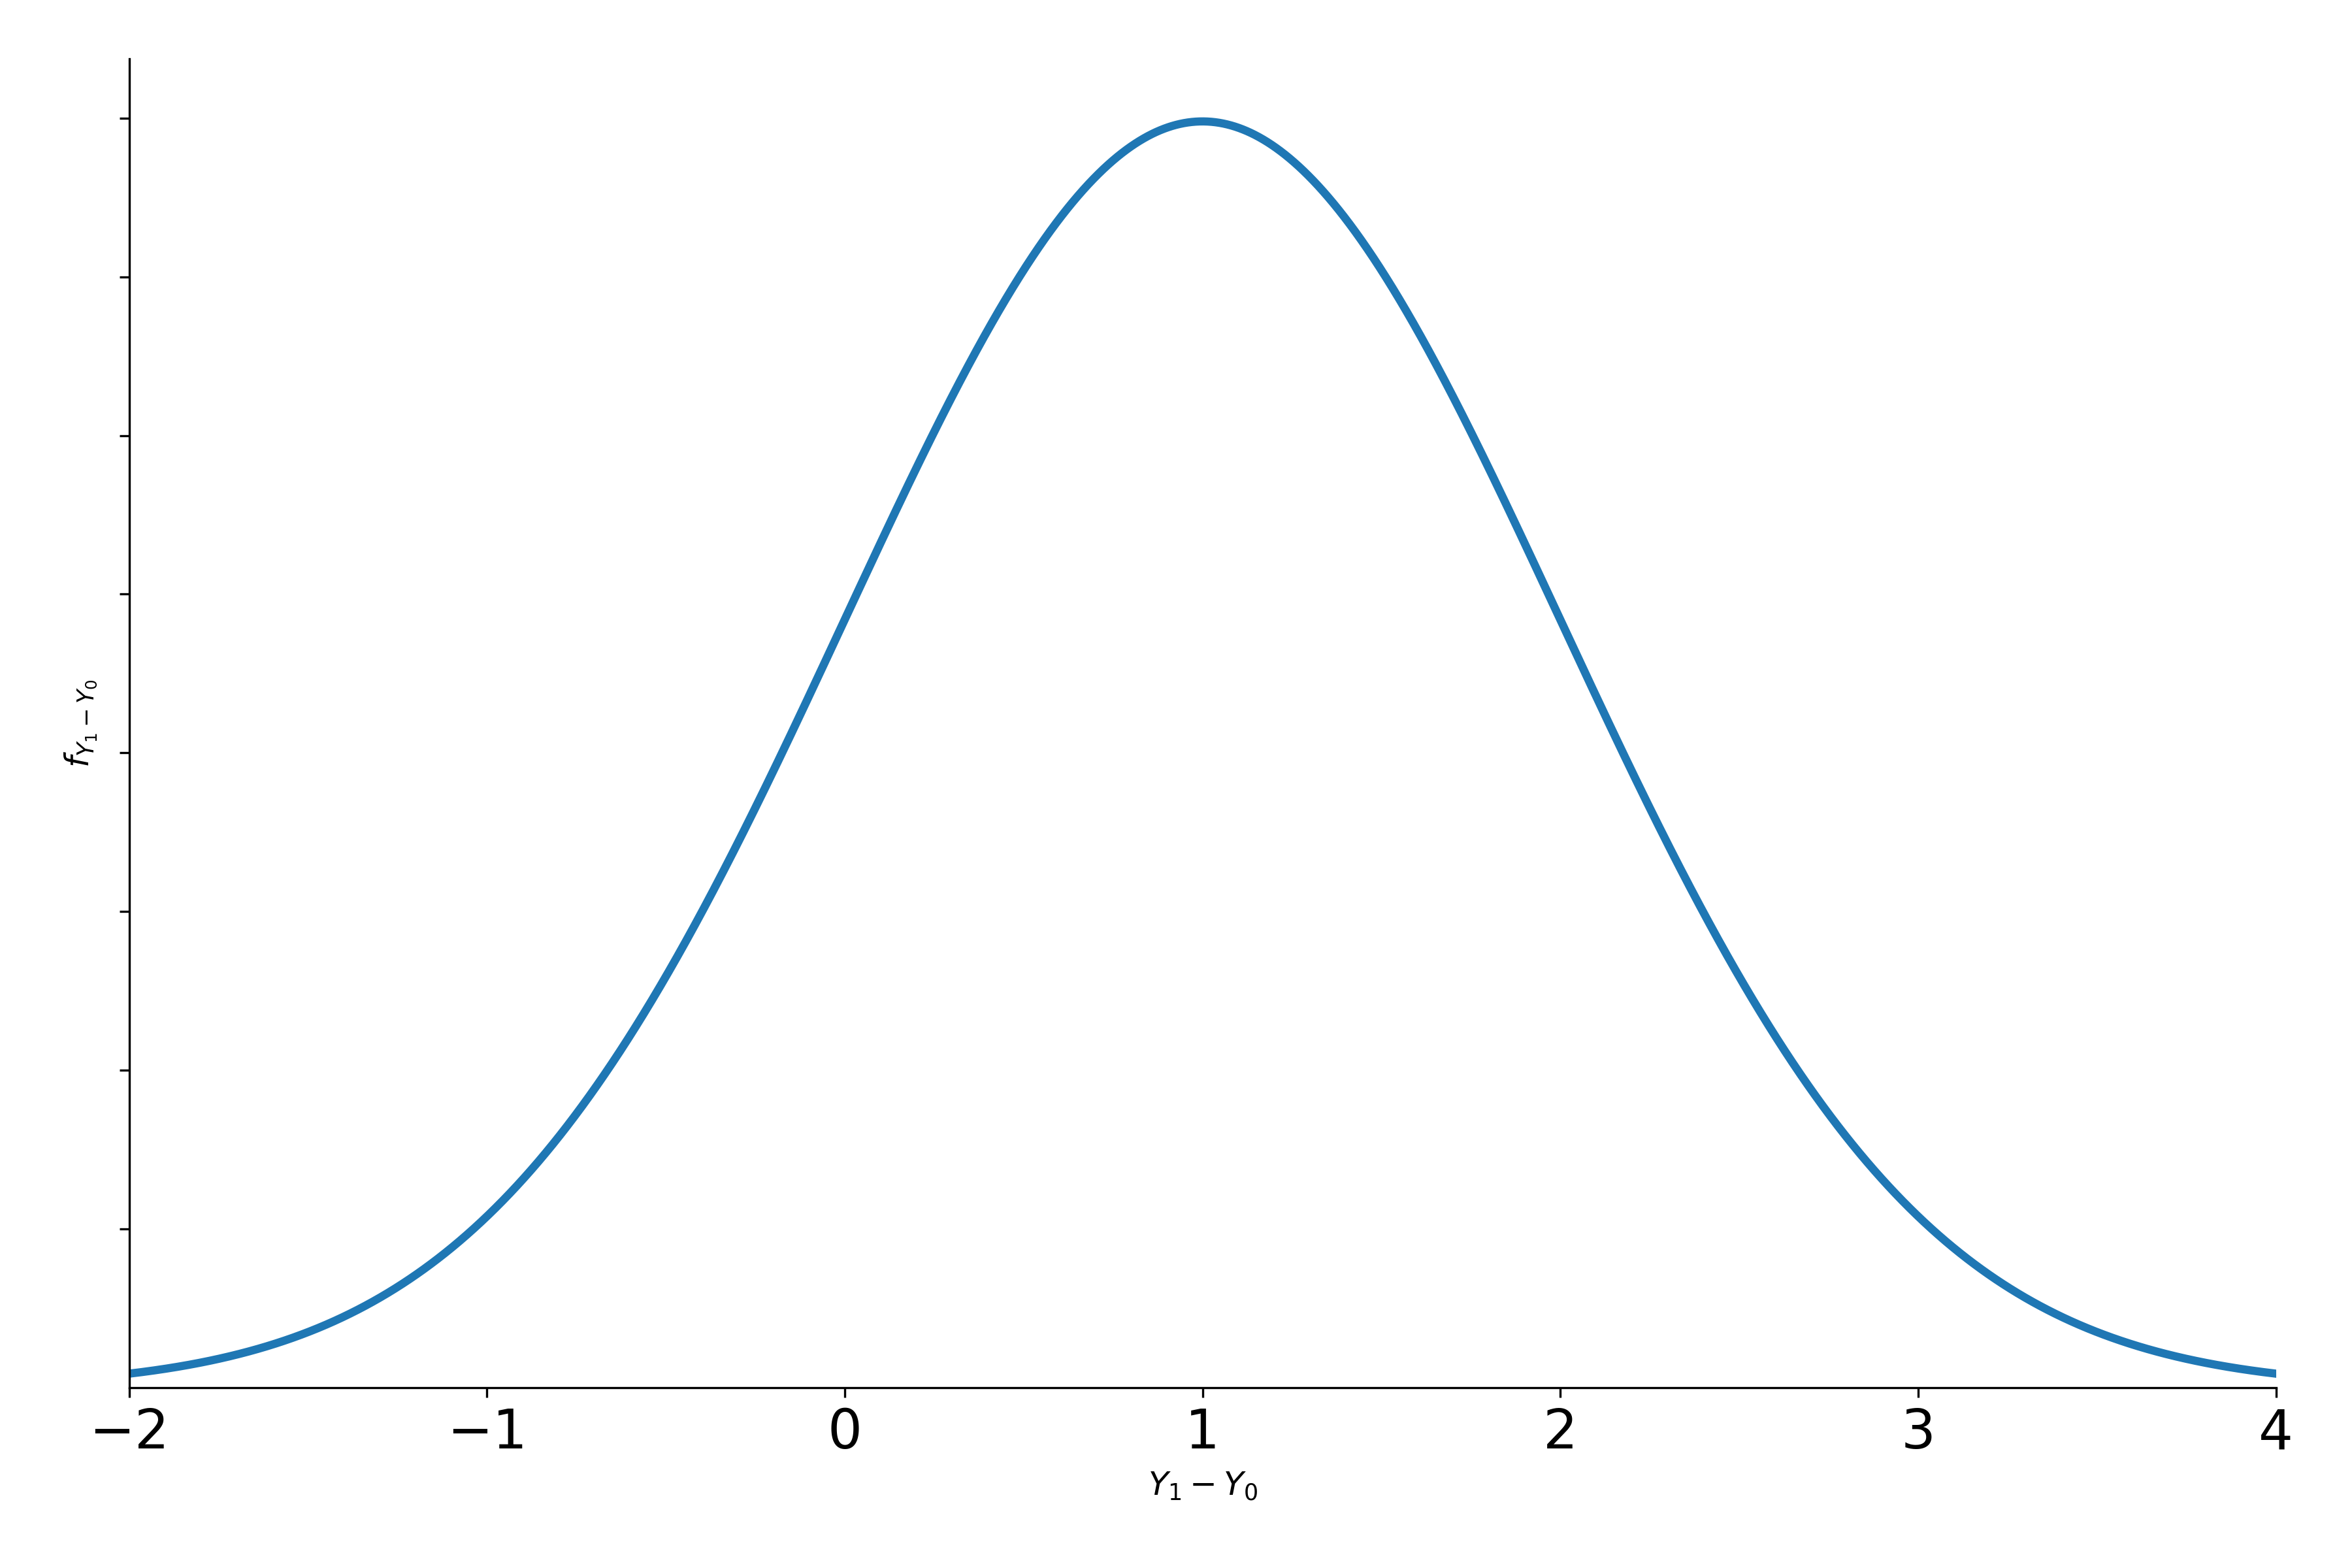
\includegraphics{fig-static-model-distribution-canvas}}
\end{figure}

\item Define and describe the marginal benefit of treatment. What exactly is the conditioning set? Complete the empty canvas below by sketching the marginal benefit of treatment in the presence and absence of essential heterogeneity. Ensure that both axes are properly labeled.

\begin{figure}[htp]\centering
\caption{Marginal benefit of treatment}\scalebox{0.35}
{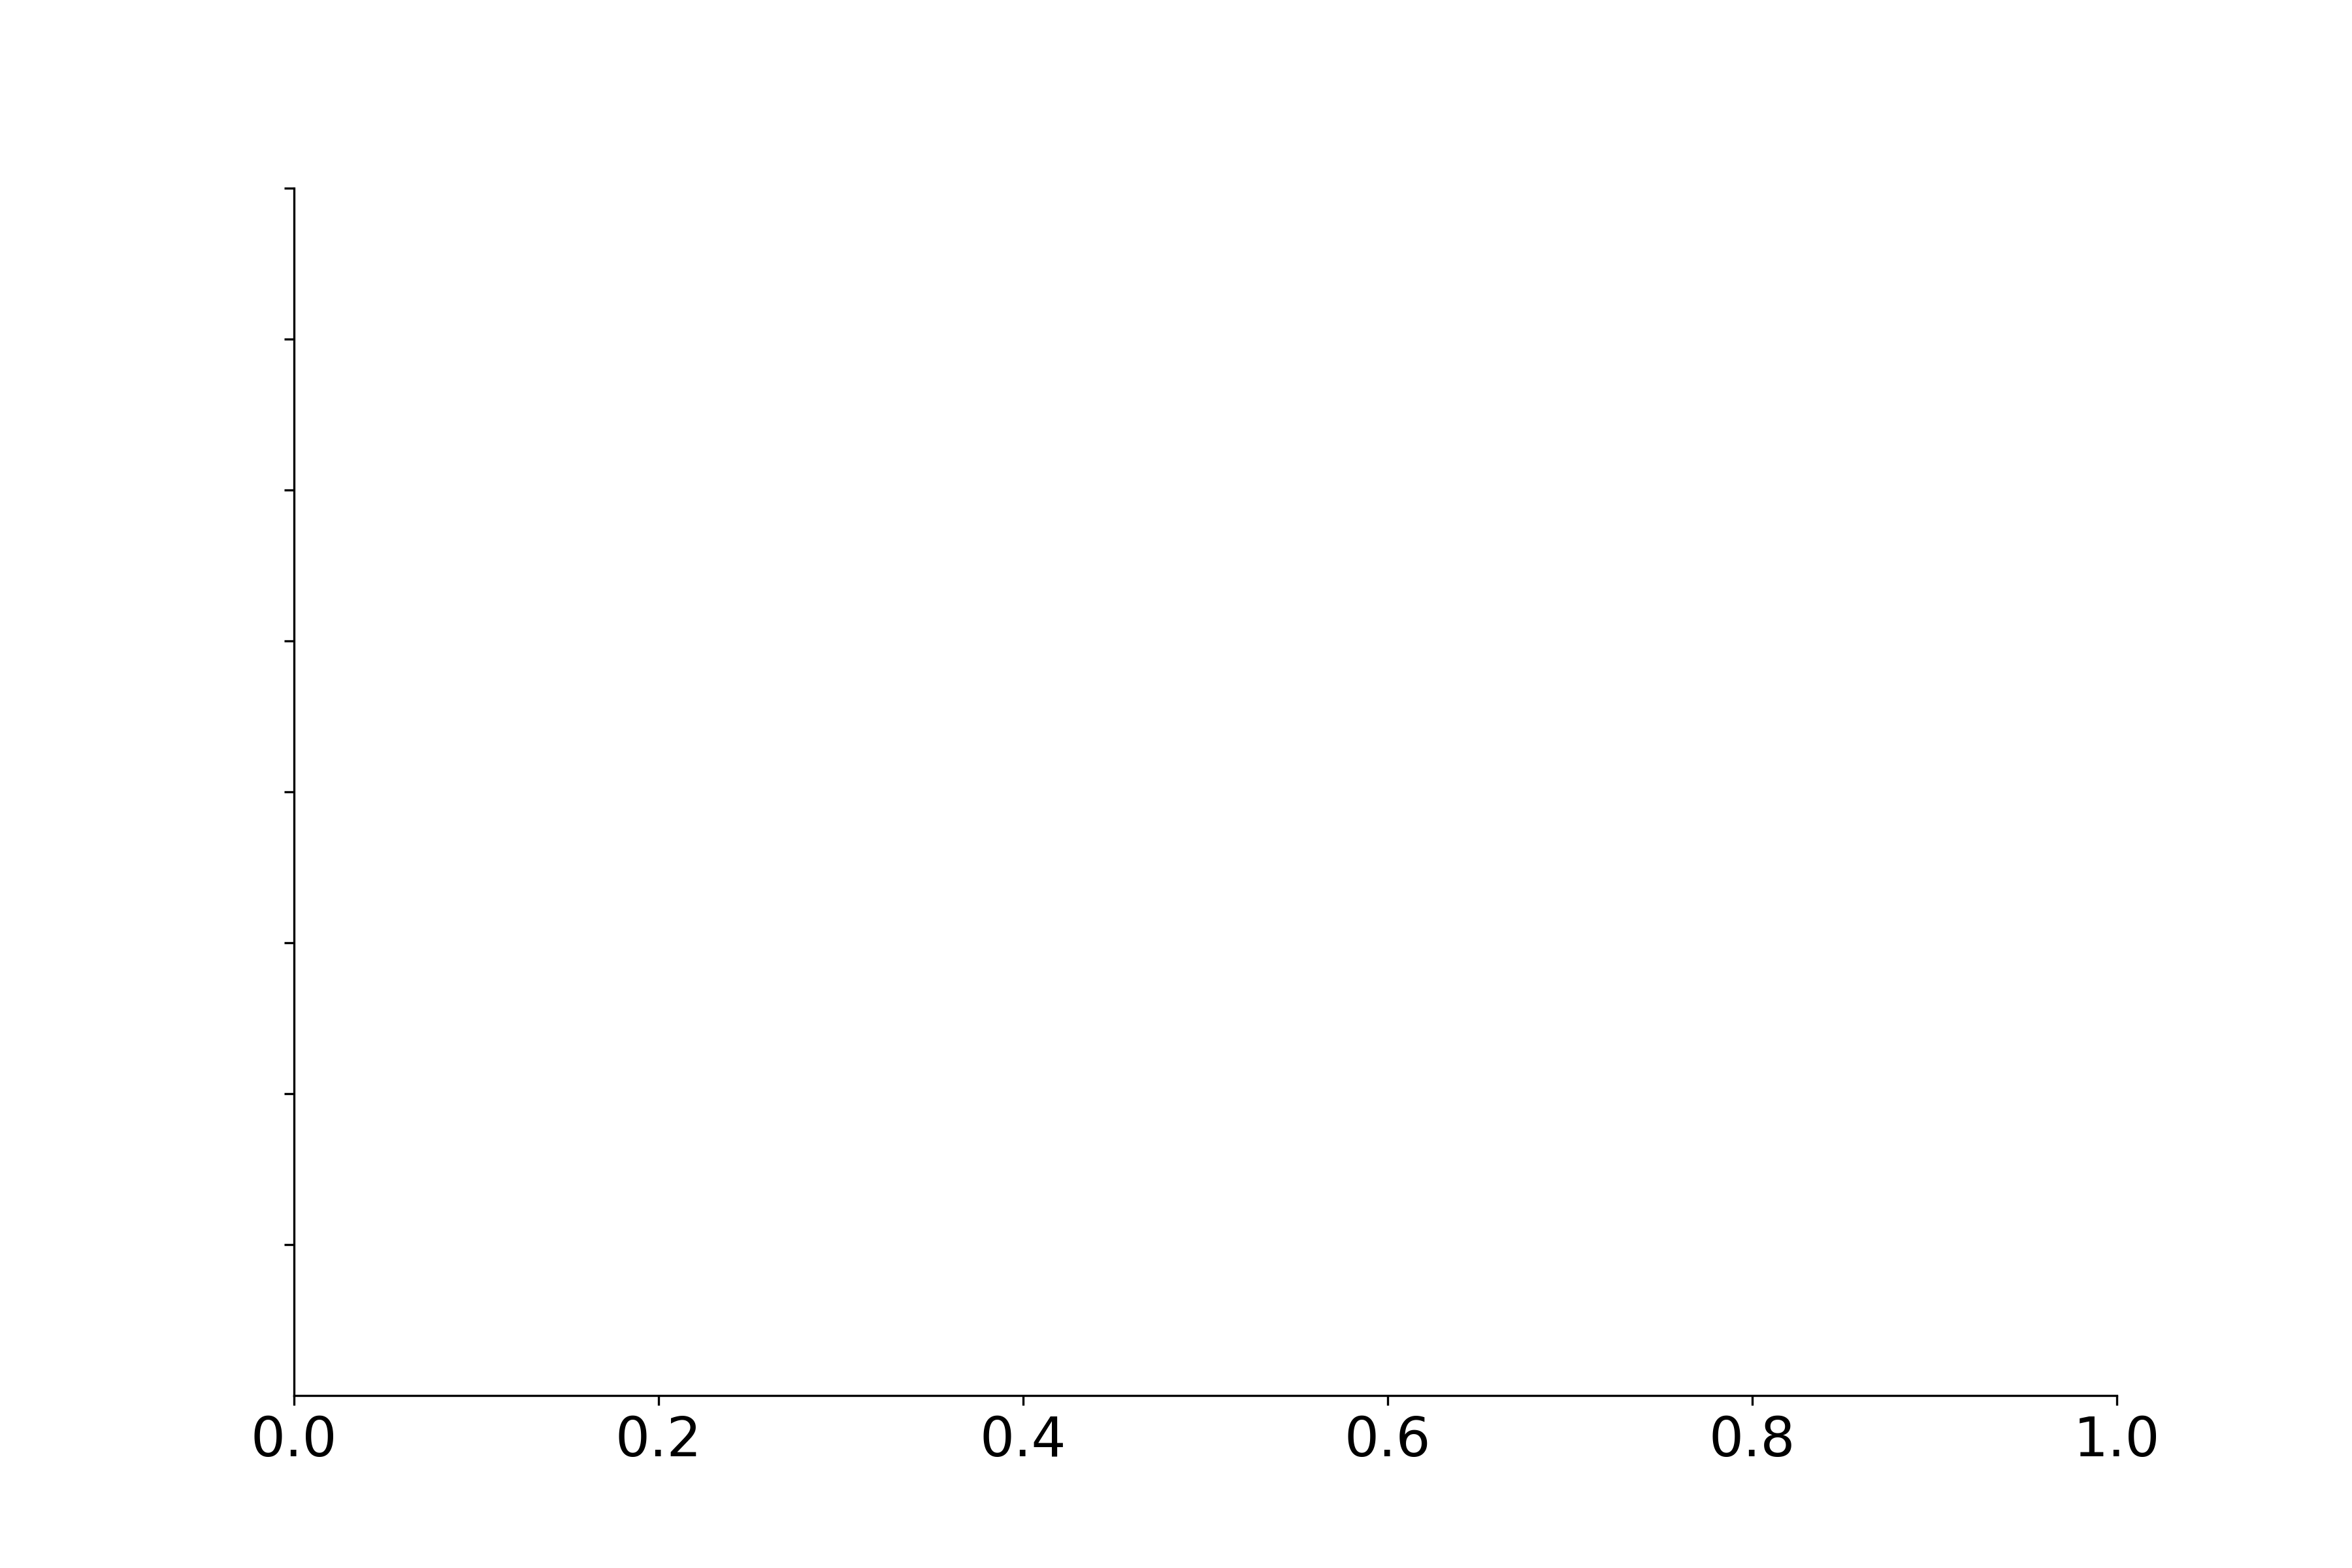
\includegraphics{fig-static-model-marginal-benefit-canvas}}
\end{figure}

\item What are the main findings in \cite{Carneiro.2011} on the marginal benefit of a college education?

\item Briefly outline the shortcomings of a static model of educational choice compared to a dynamic model.
\end{boenumerate}

Consider the following parameterization of the generalized Roy model presented in class for the static analysis of educational choice.

\begin{align*}
Y_1 & = 0.25     & D = \mathbbm{1}[\,0.50 > U\,] \\
Y_0 & = U &
\end{align*}

Assume that $U$ is unobservable and follows a uniform distribution between zero and one. Please be careful about correctly labeling all graphs that you decide to include in your answers.

\begin{boenumerate}

\item Define the individual effect of treatment. What are the sources of heterogeneity in the model. What fraction of individuals have a positive benefit of treatment?  How many do select into treatment?

\item Formally define the conventional average treatment effects and describe their limited policy relevance. How does the distribution of benefits for the model above look like? What is its exact range? Please mark the part of the distribution conditional on treatment status. Calculate the conventional effects of treatment.

\item Define and describe the concept of essential heterogeneity. Does the parameterized model exhibit essential heterogeneity? Please explain your answer.

\item Define and describe the marginal benefit of treatment $B^{MTE}$. How exactly does the $B^{MTE}$ for the parameterized model above look like?

\end{boenumerate}
